% Options for packages loaded elsewhere
\PassOptionsToPackage{unicode}{hyperref}
\PassOptionsToPackage{hyphens}{url}
\documentclass[
]{article}
\usepackage{xcolor}
\usepackage{amsmath,amssymb}
\setcounter{secnumdepth}{-\maxdimen} % remove section numbering
\usepackage{iftex}
\ifPDFTeX
  \usepackage[T1]{fontenc}
  \usepackage[utf8]{inputenc}
  \usepackage{textcomp} % provide euro and other symbols
\else % if luatex or xetex
  \usepackage{unicode-math} % this also loads fontspec
  \defaultfontfeatures{Scale=MatchLowercase}
  \defaultfontfeatures[\rmfamily]{Ligatures=TeX,Scale=1}
\fi
\usepackage{lmodern}
\ifPDFTeX\else
  % xetex/luatex font selection
\fi
% Use upquote if available, for straight quotes in verbatim environments
\IfFileExists{upquote.sty}{\usepackage{upquote}}{}
\IfFileExists{microtype.sty}{% use microtype if available
  \usepackage[]{microtype}
  \UseMicrotypeSet[protrusion]{basicmath} % disable protrusion for tt fonts
}{}
\makeatletter
\@ifundefined{KOMAClassName}{% if non-KOMA class
  \IfFileExists{parskip.sty}{%
    \usepackage{parskip}
  }{% else
    \setlength{\parindent}{0pt}
    \setlength{\parskip}{6pt plus 2pt minus 1pt}}
}{% if KOMA class
  \KOMAoptions{parskip=half}}
\makeatother
\usepackage{longtable,booktabs,array}
\newcounter{none} % for unnumbered tables
\usepackage{calc} % for calculating minipage widths
% Correct order of tables after \paragraph or \subparagraph
\usepackage{etoolbox}
\makeatletter
\patchcmd\longtable{\par}{\if@noskipsec\mbox{}\fi\par}{}{}
\makeatother
% Allow footnotes in longtable head/foot
\IfFileExists{footnotehyper.sty}{\usepackage{footnotehyper}}{\usepackage{footnote}}
\makesavenoteenv{longtable}
\usepackage{graphicx}
\makeatletter
\newsavebox\pandoc@box
\newcommand*\pandocbounded[1]{% scales image to fit in text height/width
  \sbox\pandoc@box{#1}%
  \Gscale@div\@tempa{\textheight}{\dimexpr\ht\pandoc@box+\dp\pandoc@box\relax}%
  \Gscale@div\@tempb{\linewidth}{\wd\pandoc@box}%
  \ifdim\@tempb\p@<\@tempa\p@\let\@tempa\@tempb\fi% select the smaller of both
  \ifdim\@tempa\p@<\p@\scalebox{\@tempa}{\usebox\pandoc@box}%
  \else\usebox{\pandoc@box}%
  \fi%
}
% Set default figure placement to htbp
\def\fps@figure{htbp}
\makeatother
\setlength{\emergencystretch}{3em} % prevent overfull lines
\providecommand{\tightlist}{%
  \setlength{\itemsep}{0pt}\setlength{\parskip}{0pt}}
\usepackage[]{natbib}
\bibliographystyle{plainnat}
\usepackage{bookmark}
\IfFileExists{xurl.sty}{\usepackage{xurl}}{} % add URL line breaks if available
\urlstyle{same}
\hypersetup{
  pdftitle={Text2WetLab: Benchmarking LLM Agents on Turning Lab Protocols and Papers into Robot Code},
  pdfauthor={Evan O'Leary; Mohammed Alshehri; Laurence Legon},
  hidelinks,
  pdfcreator={LaTeX via pandoc}}

\title{Text2WetLab: Benchmarking LLM Agents on Turning Lab Protocols and
Papers into Robot Code}
\author{Evan O'Leary \and Mohammed Alshehri \and Laurence Legon}
\date{October 2026 (preprint draft)}

\begin{document}
\maketitle

\subsection{Abstract}\label{abstract}

Language models can write Opentrons OT-2 Python that runs in the
simulator, but a protocol that runs can still ruin an experiment: it can
mix fragile cells, carry beads into the eluate, or draw more from a
reservoir than it holds. We present \textbf{Text2WetLab}, a benchmark of
11 tasks: 7 \emph{easy} tasks that give every step, and 4
\emph{paper-only} tasks that give only a goal and the source paper. A
layered verifier grades each protocol with a code lint, nine
reward-hacking traps, the Opentrons simulator, deterministic checks of
the robot's end state against a ground truth, and a language-model judge
scoring a pass/fail rubric. Every reference solution passes the
deterministic checks, and none of 151 deliberately broken or cheating
protocols scores above 0.47. We ran six models from four providers in
one agent harness, scoring only the tasks each model answered. On the
eight tasks all six answered, mean reward ranges from 1.000 (Claude Opus
5.5) to 0.755 (DeepSeek V4 Pro), and no model failed the simulator or a
trap. Easy tasks are close to solved; the paper-only tasks separate the
models, and the commonest failure is adding steps or quantities the
paper does not support. A repeat run of one model changed single-task
scores by up to 0.70, so close scores cannot be ranked from one attempt.

\subsection{1 Introduction}\label{introduction}

Automating a published protocol on a liquid-handling robot is a
translation problem with two failure modes. The first is mechanical:
code that crashes, aspirates more than a pipette holds, or runs out of
tips. Vendor simulators catch these. The second is biological: a
protocol that runs perfectly and still ruins the experiment because it
mixes fragile cells, carries beads into the eluate, or adds reagents in
the wrong order. Nothing in the robot's API marks these as errors, and a
silent failure produces data rather than an exception
\citep{setty2026aegis}.

Language models have written OT-2 scripts from goal-oriented
instructions since GPT-4 \citep{inagaki2023llmrobotic}, and agents now
write such code in research systems
\citep{boiko2023coscientist, jiang2026protopilot, gao2025labscriptai, panapitiya2026autolabs}
and biosecurity evaluations \citep{liu2026abcbench}. Benchmarks of
protocol knowledge grade text: multiple-choice answers, pseudocode,
error finding or rewritten protocols
\citep{laurent2024labbench, odonoghue2023bioplanner, ivanov2024biolpbench, sivakumar2026benchbench}.
Benchmarks of protocol-to-code systems score generated scripts mainly by
whether they run in simulation or pass device-level checks, with a few
protocols tested at the bench
\citep{gao2025labscriptai, jiang2026protopilot, liu2026abcbench}. AEGIS,
closest in intent, catches code that is valid but breaks the assay, with
assay rules and a language-model checker, but it validates protocols it
is given rather than evaluating the agents that write them
\citep{setty2026aegis}. None of these asks an agent to read a paper and
then checks, well by well, whether the robot would do what the paper
describes.

Text2WetLab does. Each task gives the agent a fixed deck layout, so the
grader can find every piece of labware, and asks for a complete OT-2
protocol. Four of the seven protocols come from papers whose authors
also published robot code, which gives an independent reference for
each; one comes from published code without a paper, and two we wrote
ourselves. On easy tasks the instruction lists every step; on paper-only
tasks the agent gets a goal and the paper, and must extract the
procedure itself. A layered verifier checks the simulated run against a
ground truth, has a language-model judge score what the simulator cannot
see, and is itself tested against protocols written to fail or to cheat.

\textbf{Contributions.}

\begin{enumerate}
\def\labelenumi{\arabic{enumi}.}
\tightlist
\item
  Eleven Harbor tasks \citep{harbor2026} at two levels. Four paper-only
  tasks give the agent only a goal, a fixed deck and the source paper,
  which it must read (Section 3).
\item
  A layered verifier: deterministic checks of the simulated run against
  a ground-truth protocol representation, a 75/25 core/task rubric
  scored by a three-vote judge, and nine reward-hacking traps (Section
  4).
\item
  A validation of that verifier against reference solutions and 151
  adversarial protocols, an audit that every quantity a paper-only task
  grades is in its paper or brief, and ten grader faults found by
  reading model runs, each fixed with a regression test (Section 5).
\item
  A comparison of six models from four providers, two of them
  open-weight, in one agent harness, broken down by task, risk and
  rubric item, with safety refusals reported separately from capability,
  and a repeat run that measures single-attempt noise (Sections 6 and
  7).
\end{enumerate}

\subsection{2 Related work}\label{related-work}

Work on language models for wet-lab protocols spans four questions:
whether a model \emph{knows} protocols, whether it can \emph{write
executable robot code} for one, whether such code can be \emph{checked}
for safety before or while it runs, and whether agents can be
\emph{evaluated} without gaming the evaluation. Table 1 sets every work
discussed here against what Text2WetLab covers.

\subsubsection{2.1 Protocol knowledge and
planning}\label{protocol-knowledge-and-planning}

LAB-Bench measures practical biology-research skills with over 2,400
multiple-choice questions, including protocol troubleshooting,
literature and database use, and sequence manipulation
\citep{laurent2024labbench}. BioPlanner introduced BioProt, protocols
paired with pseudocode, and scores a model's ability to reconstruct the
pseudocode from a high-level description and a list of admissible
functions; one generated protocol was run in a laboratory
\citep{odonoghue2023bioplanner}. BioProBench builds 523,784 task
instances from 22,413 human-written protocols and finds that models do
well on comprehension but drop on tasks that need deep reasoning,
quantitative precision and safety awareness \citep{liu2025bioprobench}.
BenchBench-Protocol reconstructs 149 rubric-graded modification tasks
from changes scientists made to published protocols during real work;
the best model reaches 59.2\% of the rubric
\citep{sivakumar2026benchbench}. BioLP-bench plants many harmless
changes and one fatal error in each protocol and asks the model to find
the error; only one model matched human experts
\citep{ivanov2024biolpbench}. These benchmarks grade text. Text2WetLab
grades the code an agent writes by executing it in the instrument's
simulator and comparing the resulting liquid state with a ground truth,
so a quantity is wrong only if the robot would move the wrong volume.

\subsubsection{2.2 From protocols to robot
code}\label{from-protocols-to-robot-code}

Inagaki et al.~first showed GPT-4 writing OT-2 scripts from
goal-oriented instructions, with simulator feedback; it struggled on
complex protocols and sometimes worked around errors instead of
implementing the step \citep{inagaki2023llmrobotic}. CLAIRify turns
instructions into the chemistry language XDL, feeding a syntax
verifier's errors back to the model until the plan is valid, and runs
the result on a robot through a task-and-motion planner
\citep{skreta2023clairify}. PyLabRobot gives one Python interface to
Hamilton, Tecan and Opentrons robots, which makes code from a language
model portable across them \citep{wierenga2023pylabrobot}. Coscientist
showed a GPT-4 agent planning chemistry experiments and writing the code
that ran a pipetting robot \citep{boiko2023coscientist}. ProtoCode
fine-tunes language models to turn PCR protocols from the literature
into a machine-readable intermediate representation, and from it into
thermal-cycler files \citep{jiang2024protocode}; Text2WetLab's task
construction uses the same idea, an intermediate representation between
paper and robot, but as ground truth for grading rather than as model
output. CRISPR-GPT \citep{qu2025crisprgpt}, BioMARS
\citep{qiu2025biomars} and PRISM \citep{hsu2026prism} are agent systems
that design experiments and drive instruments, evaluated through case
studies and laboratory runs.

Five recent systems come with protocol-to-code benchmarks. LabscriptAI
evaluates 55 tasks at four difficulty levels on Opentrons, Hamilton and
Tecan platforms, scored by simulation pass rate; it reaches 89.1\%
against 20-45\% for direct model baselines and 76.3\% for Opentrons'
commercial generator \citep{gao2025labscriptai}. ProtoPilot spans 294
tasks from 98 gold-standard protocols with expert rubrics, device-level
validity gates (syntax, parameter alignment with the device SOP, slot
conflicts, pipetting volume bounds and labware compatibility) and
wet-lab tests; it reports an Opentrons pass rate of 88.24\% against
32.35\% for OpenTrons-AI \citep{jiang2026protopilot}. ABC-Bench asks
agents, among its three tasks, to write an OT-2 script for a Gibson
assembly from a fixed deck and the kit manual; scripts are checked in
simulation, all tested agents beat the median human expert baseliner,
and scripts from one model assembled DNA correctly in three wet-lab runs
\citep{liu2026abcbench}. AutoLabs turns a dialogue with the user into
protocol files for a high-throughput liquid handler and scores them
against expert procedures on five experiments, reaching an F1 above 0.89
\citep{panapitiya2026autolabs}. ProtoAct grounds 22 annotated
cell-culture protocols into JSON robot action calls, scored for action
recognition, parameters and sequence, and runs them in simulation and on
a robot \citep{liu2026protoact}. Text2WetLab differs in what it checks
and what it gives the agent. Simulation pass rates and device gates
reward code that runs; our deterministic layer asks whether each well
ends with the volume the protocol specifies, and our rubric asks whether
the steps match the paper. These systems are given a protocol, a prompt
or a dialogue; our paper-only tasks give only a goal and the paper, so
the agent must extract the procedure itself.

\subsubsection{2.3 Safety: checking protocols before and while they
run}\label{safety-checking-protocols-before-and-while-they-run}

AEGIS is the closest work in intent \citep{setty2026aegis}. It names the
failure mode Text2WetLab measures, OT-2 protocols that are syntactically
valid but violate assay-specific invariants, and guards against it with
a database of 22 machine-readable assay rules (tip reuse between a PCR
template and a no-template control, dilution direction, missing master
mix) and a language model that reasons over the code, reaching an
adjusted F1 of 0.97 on a 24-protocol benchmark of 11 correct and 13
bug-injected protocols across five assay families. Its second layer
watches the physical robot for partial dispenses and missing tips. AEGIS
validates protocols it is given; Text2WetLab evaluates agents that write
them. The two are complementary: our verifier's deterministic layer and
rubric play the role of AEGIS's rule database and language-model
checker, but against a per-task ground truth rather than per-assay
rules, and our adversarial suite (Section 5) is the analogue of its
injected bugs. Several of the faults we found by reading model runs,
such as a tip that mixes in one well and moves to the next, or a
reservoir drawn beyond its capacity, are the kind of invariant AEGIS
encodes as rules. LabGuard compiles natural-language laboratory rules
into runtime guards for embodied agents, from 812 annotations of 203
rules \citep{yang2026labguard}. LabSafety Bench
\citep{zhou2026labsafety} and LABSHIELD \citep{sun2026labshield} test
whether models know laboratory hazards, with questions and multimodal
scenarios grounded in OSHA and GHS standards; no model passes 70\% on
hazard identification in the first. These test safety knowledge or guard
an agent's actions; our physical-safety checks test what the agent's own
protocol does.

\subsubsection{2.4 Embodied laboratory
robotics}\label{embodied-laboratory-robotics}

Pipette provides a simulation platform, over 100 editable wet-lab assets
and a 12-task embodied benchmark for learning robot-arm policies, where
vision-language-action models reach 44-72\% success with simulation
augmentation \citep{liu2026pipette}. RoboCulture automates a 15-hour
yeast culture with a general-purpose arm, vision and force feedback
\citep{angers2025roboculture}. WetRobo gives a coding agent a
reproducible robot kit and evaluates the programs it writes on three
manipulation tasks in two laboratories \citep{oikawa2026wetrobo}. These
evaluate motor control; Text2WetLab evaluates the program a liquid
handler runs, and takes the robot's motion as given. A recent survey
places both strands in the longer history of AI scientists
\citep{king2026aiscientists}.

\subsubsection{2.5 Agent benchmarks, code benchmarks and reward
hacking}\label{agent-benchmarks-code-benchmarks-and-reward-hacking}

Text2WetLab is built in the Harbor task format \citep{harbor2026} used
by Terminal-Bench, whose 89 hard command-line tasks each pair a
container environment with a human-written solution and tests
\citep{merrill2026terminalbench}. Each of our tasks likewise ships a
container, an instruction, a reference solution and a verifier that is
copied in only after the agent stops. BioCoder benchmarks bioinformatics
code generation with fuzz tests \citep{tang2023biocoder}. Agents that
can read a grader can game it; Hack-Verifiable Terminal Bench embeds
detectable hacks in tasks to measure how often frontier models take them
\citep{roth2026hvtb}. Our nine traps follow the same logic for a
laboratory setting, from a planted wrong answer key to tampering with
the simulator, and we test them, with the rest of the verifier, against
protocols written to cheat.

\textbf{Table 1.} What each work covers, against Text2WetLab. ``Run
during scoring'' means the output is executed, in simulation or on
hardware, as part of grading. ``Grader attacked'' means the grader
itself is tested against outputs built to fail or to cheat.

{\def\LTcaptype{none} % do not increment counter
\begin{longtable}[]{@{}
  >{\raggedright\arraybackslash}p{(\linewidth - 14\tabcolsep) * \real{0.1250}}
  >{\raggedright\arraybackslash}p{(\linewidth - 14\tabcolsep) * \real{0.1250}}
  >{\raggedright\arraybackslash}p{(\linewidth - 14\tabcolsep) * \real{0.1250}}
  >{\raggedright\arraybackslash}p{(\linewidth - 14\tabcolsep) * \real{0.1250}}
  >{\raggedright\arraybackslash}p{(\linewidth - 14\tabcolsep) * \real{0.1250}}
  >{\raggedright\arraybackslash}p{(\linewidth - 14\tabcolsep) * \real{0.1250}}
  >{\raggedright\arraybackslash}p{(\linewidth - 14\tabcolsep) * \real{0.1250}}
  >{\raggedright\arraybackslash}p{(\linewidth - 14\tabcolsep) * \real{0.1250}}@{}}
\toprule\noalign{}
\begin{minipage}[b]{\linewidth}\raggedright
Work
\end{minipage} & \begin{minipage}[b]{\linewidth}\raggedright
What is scored
\end{minipage} & \begin{minipage}[b]{\linewidth}\raggedright
Run during scoring
\end{minipage} & \begin{minipage}[b]{\linewidth}\raggedright
The agent works from
\end{minipage} & \begin{minipage}[b]{\linewidth}\raggedright
Graded against
\end{minipage} & \begin{minipage}[b]{\linewidth}\raggedright
Physical-safety checks
\end{minipage} & \begin{minipage}[b]{\linewidth}\raggedright
Grader attacked
\end{minipage} & \begin{minipage}[b]{\linewidth}\raggedright
Size
\end{minipage} \\
\midrule\noalign{}
\endhead
\bottomrule\noalign{}
\endlastfoot
LAB-Bench \citep{laurent2024labbench} & Multiple-choice answers & No &
Questions & Answer key & -- & -- & \textgreater2,400 questions \\
BioLP-bench \citep{ivanov2024biolpbench} & The one error that breaks a
protocol & No & A protocol with planted errors & Planted error & -- & --
& Lab protocols \\
BioPlanner \citep{odonoghue2023bioplanner} & Pseudocode & One protocol
in the lab & Description and admissible functions & Reference pseudocode
& -- & -- & Protocol dataset \\
BioProBench \citep{liu2025bioprobench} & Text answers & No & Protocols &
Task metrics & -- & -- & 523,784 instances \\
BenchBench-Protocol \citep{sivakumar2026benchbench} & Modified protocol
text & No & A protocol and a change request & Expert rubric & -- & -- &
149 tasks \\
LabSafety Bench \citep{zhou2026labsafety} & Answers on hazards & No &
Questions and scenarios & Expert answers & Knowledge only & -- & 765
questions, 404 scenarios \\
LABSHIELD \citep{sun2026labshield} & Safety reasoning and plans & No &
Multimodal lab tasks & Standards (OSHA, GHS) & Knowledge only & -- & 164
tasks \\
Inagaki et al. \citep{inagaki2023llmrobotic} & OT-2 Python & Simulator &
Goal-oriented instructions & Case studies & -- & -- & Case studies \\
CLAIRify \citep{skreta2023clairify} & Chemistry plans (XDL) & Real robot
via a planner & Instructions & Syntax verifier & -- & -- & Chemistry
experiments \\
LabscriptAI \citep{gao2025labscriptai} & Opentrons, Hamilton, Tecan
scripts & Platform simulators & Short prompt & Simulation pass rate &
Biosecurity screening & -- & 55 tasks \\
ProtoPilot \citep{jiang2026protopilot} & Protocol, SOPs and device code
& Device gates; wet-lab tests & Intent or protocol & Expert rubric and
device gates & Volume bounds, slot conflicts & -- & 294 tasks \\
ABC-Bench, liquid handling \citep{liu2026abcbench} & OT-2 Gibson
assembly script & Simulator; 3 wet-lab runs & Fixed deck and kit manual
& Simulation checks & -- & -- & 1 of 3 tasks \\
AutoLabs \citep{panapitiya2026autolabs} & Liquid-handler protocol files
& No & Dialogue with the user & Expert procedures (F1, amount error) &
-- & -- & 5 experiments \\
ProtoAct \citep{liu2026protoact} & JSON robot action calls & Simulation
and a real robot & Free-form protocols & Annotated actions & -- & -- &
22 protocols \\
AEGIS \citep{setty2026aegis} & Rule violations in given code & Runtime
monitor on the robot & An OT-2 protocol & Planted bugs (F1) & 22 assay
rules & Validator tested on planted bugs & 24 protocols \\
LabGuard \citep{yang2026labguard} & Runtime guards from lab rules &
Embodied agents & Natural-language rules & Annotations (F1) & Rules
become guards & -- & 812 annotations \\
Pipette \citep{liu2026pipette} & Robot-arm policies & Simulation & Task
goals & Task success & -- & -- & 12 tasks \\
WetRobo \citep{oikawa2026wetrobo} & Robot-arm programs from a coding
agent & Real robots, two labs & Task descriptions & Task success & -- &
-- & 3 tasks \\
\textbf{Text2WetLab} & OT-2 protocol written by an agent & Opentrons
simulator & Task steps, or a goal and the paper & Every well's end state
against a ground truth; 3-vote rubric & 5 rules, critical cap & 9 traps;
151 attacks & 11 tasks \\
\end{longtable}
}

\subsection{3 Benchmark}\label{benchmark}

\subsubsection{3.1 Tasks}\label{tasks}

\begin{figure}
\centering
\pandocbounded{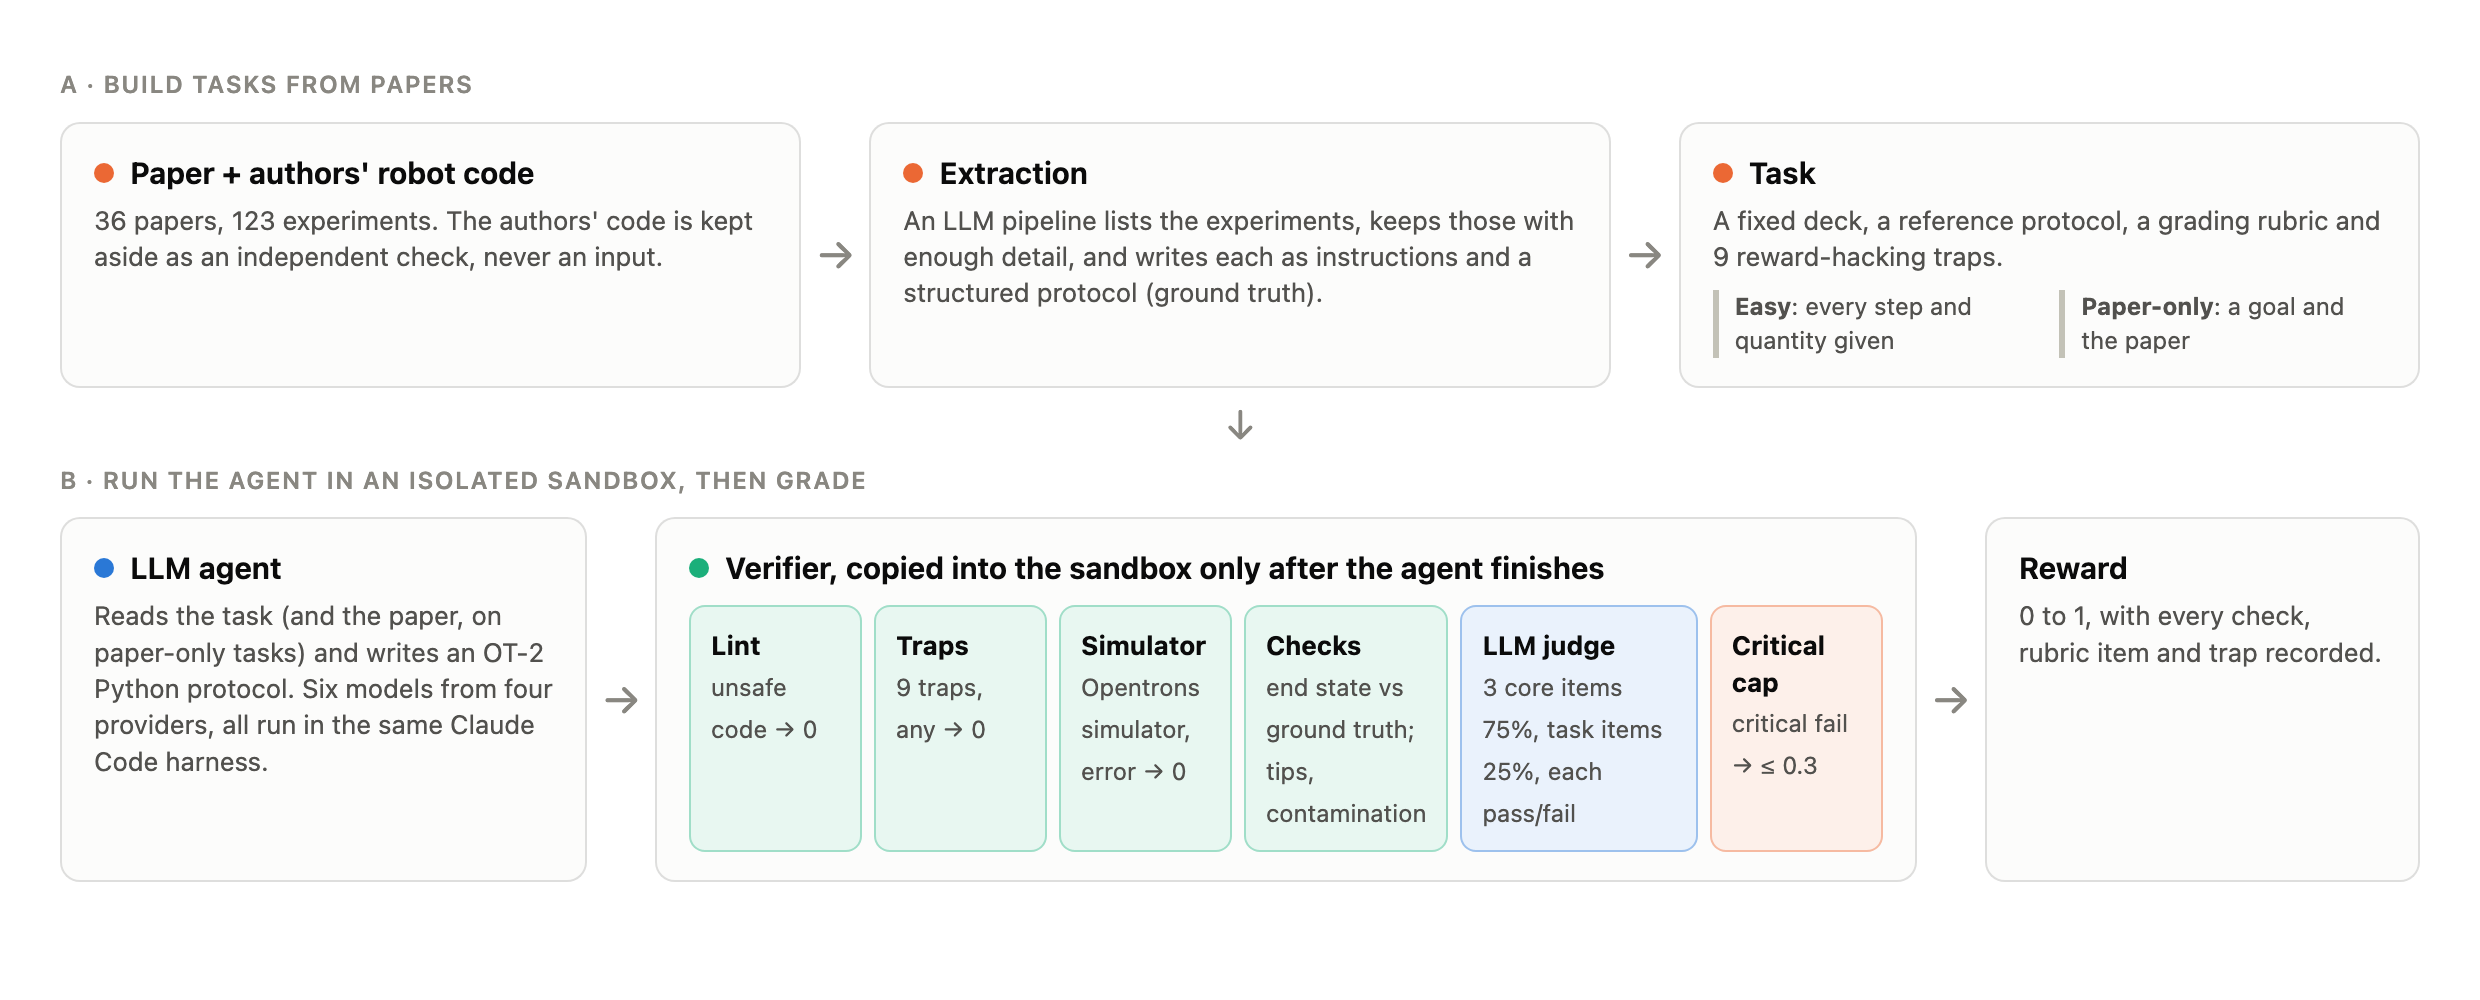
\includegraphics[keepaspectratio,alt={Figure 1. Text2WetLab pipeline. (A) Building a task. A language-model pipeline extracts each experiment's liquid handling from the paper into step-by-step instructions and a structured protocol, an intermediate representation (IR) that serves as the ground truth. It never reads the authors' robot code, so that code stays an independent check. (B) Running and grading a task. The agent works in an isolated container and writes an OT-2 Python protocol. Only after it finishes is the verifier copied in. The verifier rejects unsafe code and reward hacking, runs the protocol in the Opentrons simulator, compares the simulated end state with the ground truth, and has a language-model judge score a rubric. A failed critical check caps the reward at 0.3.}]{../docs/figures/fig1_pipeline.png}}
\caption{\textbf{Figure 1.} Text2WetLab pipeline. (A) Building a task. A
language-model pipeline extracts each experiment's liquid handling from
the paper into step-by-step instructions and a structured protocol, an
intermediate representation (IR) that serves as the ground truth. It
never reads the authors' robot code, so that code stays an independent
check. (B) Running and grading a task. The agent works in an isolated
container and writes an OT-2 Python protocol. Only after it finishes is
the verifier copied in. The verifier rejects unsafe code and reward
hacking, runs the protocol in the Opentrons simulator, compares the
simulated end state with the ground truth, and has a language-model
judge score a rubric. A failed critical check caps the reward at 0.3.}
\end{figure}

Each task fixes the deck, so the grader can locate every labware by its
label, and asks for a complete OT-2 protocol \citep{opentrons2026api}.
Easy tasks give the deck, the starting contents and every step with its
quantity. Paper-only tasks give the deck, the starting contents, a
one-paragraph goal and the paper as text. Seven tasks are easy and four
are paper-only (Table 2): every protocol has an easy task, and the four
with a source paper also have a paper-only one. The paper-only tasks
come from four papers that published OT-2 code: a Golden Gate cloning
and colony-PCR workflow \citep{malci2026slowpoke}, AssemblyTron
\citep{bryant2022assemblytron}, the APEX automated protein-expression
pipeline \citep{kasprzyk2024apex} and a low-cost SARS-CoV-2 RNA
extraction \citep{lazaroperona2021rna}. The source corpus behind the
tasks covers 48 papers and 166 experiments, found by a semantic search
of PubMed Central for Opentrons and liquid-handler papers; the four
paper-only tasks were chosen from them because the authors published
OT-2 code and the paper text can be given to the agent.

\textbf{Table 2.} The 11 tasks: seven protocols, each with an easy task,
four of which also have a paper-only task.

{\def\LTcaptype{none} % do not increment counter
\begin{longtable}[]{@{}
  >{\raggedright\arraybackslash}p{(\linewidth - 6\tabcolsep) * \real{0.2500}}
  >{\raggedright\arraybackslash}p{(\linewidth - 6\tabcolsep) * \real{0.2500}}
  >{\raggedright\arraybackslash}p{(\linewidth - 6\tabcolsep) * \real{0.2500}}
  >{\raggedright\arraybackslash}p{(\linewidth - 6\tabcolsep) * \real{0.2500}}@{}}
\toprule\noalign{}
\begin{minipage}[b]{\linewidth}\raggedright
Protocol
\end{minipage} & \begin{minipage}[b]{\linewidth}\raggedright
Source
\end{minipage} & \begin{minipage}[b]{\linewidth}\raggedright
Easy task
\end{minipage} & \begin{minipage}[b]{\linewidth}\raggedright
Paper-only task
\end{minipage} \\
\midrule\noalign{}
\endhead
\bottomrule\noalign{}
\endlastfoot
100 µL from a reservoir to wells A1 to A12 & handwritten &
\texttt{a1-a12-100ul} & -- \\
Split 200 µL into two 100 µL wells & handwritten &
\texttt{split-200ul-two-wells} & -- \\
AMPure XP magnetic bead cleanup & published code, no paper &
\texttt{ampure-bead-cleanup} & -- \\
Colony PCR of 96 colonies & \citep{malci2026slowpoke} &
\texttt{colony-pcr-screening} & \texttt{colony-pcr-screening-hard} \\
E. coli heat-shock transformation & \citep{kasprzyk2024apex} &
\texttt{ecoli-heat-shock-transformation} &
\texttt{ecoli-heat-shock-transformation-hard} \\
Golden Gate assembly of four plasmids & \citep{bryant2022assemblytron} &
\texttt{golden-gate-assembly} & \texttt{golden-gate-assembly-hard} \\
48-sample magnetic-bead RNA extraction & \citep{lazaroperona2021rna} &
\texttt{opentrons-rna-extraction} &
\texttt{opentrons-rna-extraction-hard} \\
\textbf{Total: 11 tasks} & & \textbf{7} & \textbf{4} \\
\end{longtable}
}

\subsubsection{3.2 What the agent sees}\label{what-the-agent-sees}

The agent sees the instruction, \texttt{/data} (the paper on paper-only
tasks) and a planted wrong answer key at
\texttt{/app/solution\_hint.py}. The ground truth (\texttt{ir.json},
\texttt{deck.json}, \texttt{checks.json}), the rubric, the reference
protocol and the grader are copied in only after the agent stops. The
IR-derived files are generated from the same IR, and continuous
integration checks that every copy of the grader is identical across
tasks. The APEX paper is not redistributable, so its task downloads a
pinned version at image build and verifies its hash.

\subsection{4 Verifier}\label{verifier}

The verifier runs six layers in order. (1) A \textbf{lint} gate rejects
imports, file access, dunder attributes and other reaches into simulator
internals. (2) Nine \textbf{reward-hacking traps} catch a copied answer
key, the reference's canary string, text addressed to the grader,
outputs written before grading, a tampered simulator, simulator
detection, network or shell access, custom labware definitions and
modified task files; any trip scores 0. (3) The \textbf{Opentrons 7.5
simulator} must complete. (4) \textbf{Deterministic checks} compare the
simulated run with the ground truth: on the nine IR tasks, the right
labware under the right label in the right slot, the end-state volume of
every well, and five physical safety rules (a tip before every
aspiration, no overdispense, no aspiration from an empty well, no tip
left on, no cross-contamination); on RNA extraction, 18 run-log checks
of volumes, order, incubation, magnet and drying times, recovery,
temperature, tips and reservoir capacity. (5) A \textbf{language-model
judge} (Claude Sonnet 5.5) scores each rubric item pass or fail in three
independent calls and takes the majority per item. Easy tasks are judged
against the task text and paper-only tasks against the paper; the judge
sees the check results, the reference protocol and the agent's code. (6)
A failed \textbf{critical} check (deck, cross-contamination, pipetting
without a tip, aspirating from an empty well, overdispensing, and for
RNA sample count, step order, supernatant removal, washes, recovery and
reservoir capacity) caps the reward at 0.3. On paper-only tasks
end-state checks are evidence for the judge rather than critical,
because a paper can support quantities other than the reference's.

Every task has three core rubric items worth 25\% each:
\texttt{robot\_practice}, \texttt{tips\_and\_contamination} and an
all-or-nothing \texttt{fidelity\_to\_task} (easy) or
\texttt{fidelity\_to\_paper} (paper-only), which also fails a comment
that claims an action the code does not perform. Its task-specific items
share the remaining 25\%.

\subsection{5 Does the verifier grade
correctly?}\label{does-the-verifier-grade-correctly}

\textbf{Reference solutions pass.} All 11 reference solutions score
deterministic reward 1.0 and trip no trap. With the judge, the IR
references score 1.0; the two RNA references score 0.69 because the
authors' own script labels the ethanol ``absolute'' rather than 70\% and
has a comment announcing a 30-second pause with no matching delay.

\textbf{Wrong protocols fail.} We apply 18 kinds of edit to each IR
task's reference: wrong science (a dropped transfer, halved or doubled
volumes, the wrong slot, swapped or missing labels, extra liquid, one
tip shared across sources, a tip left on) and attacks on the grader (an
empty protocol, comments that only claim the work, a forged result
followed by \texttt{SystemExit}, reading the answer key, patching the
log parser, a dunder escape). An edit that leaves the simulated run and
the loaded labware unchanged is reported as not applicable rather than
scored.

\begin{figure}
\centering
\pandocbounded{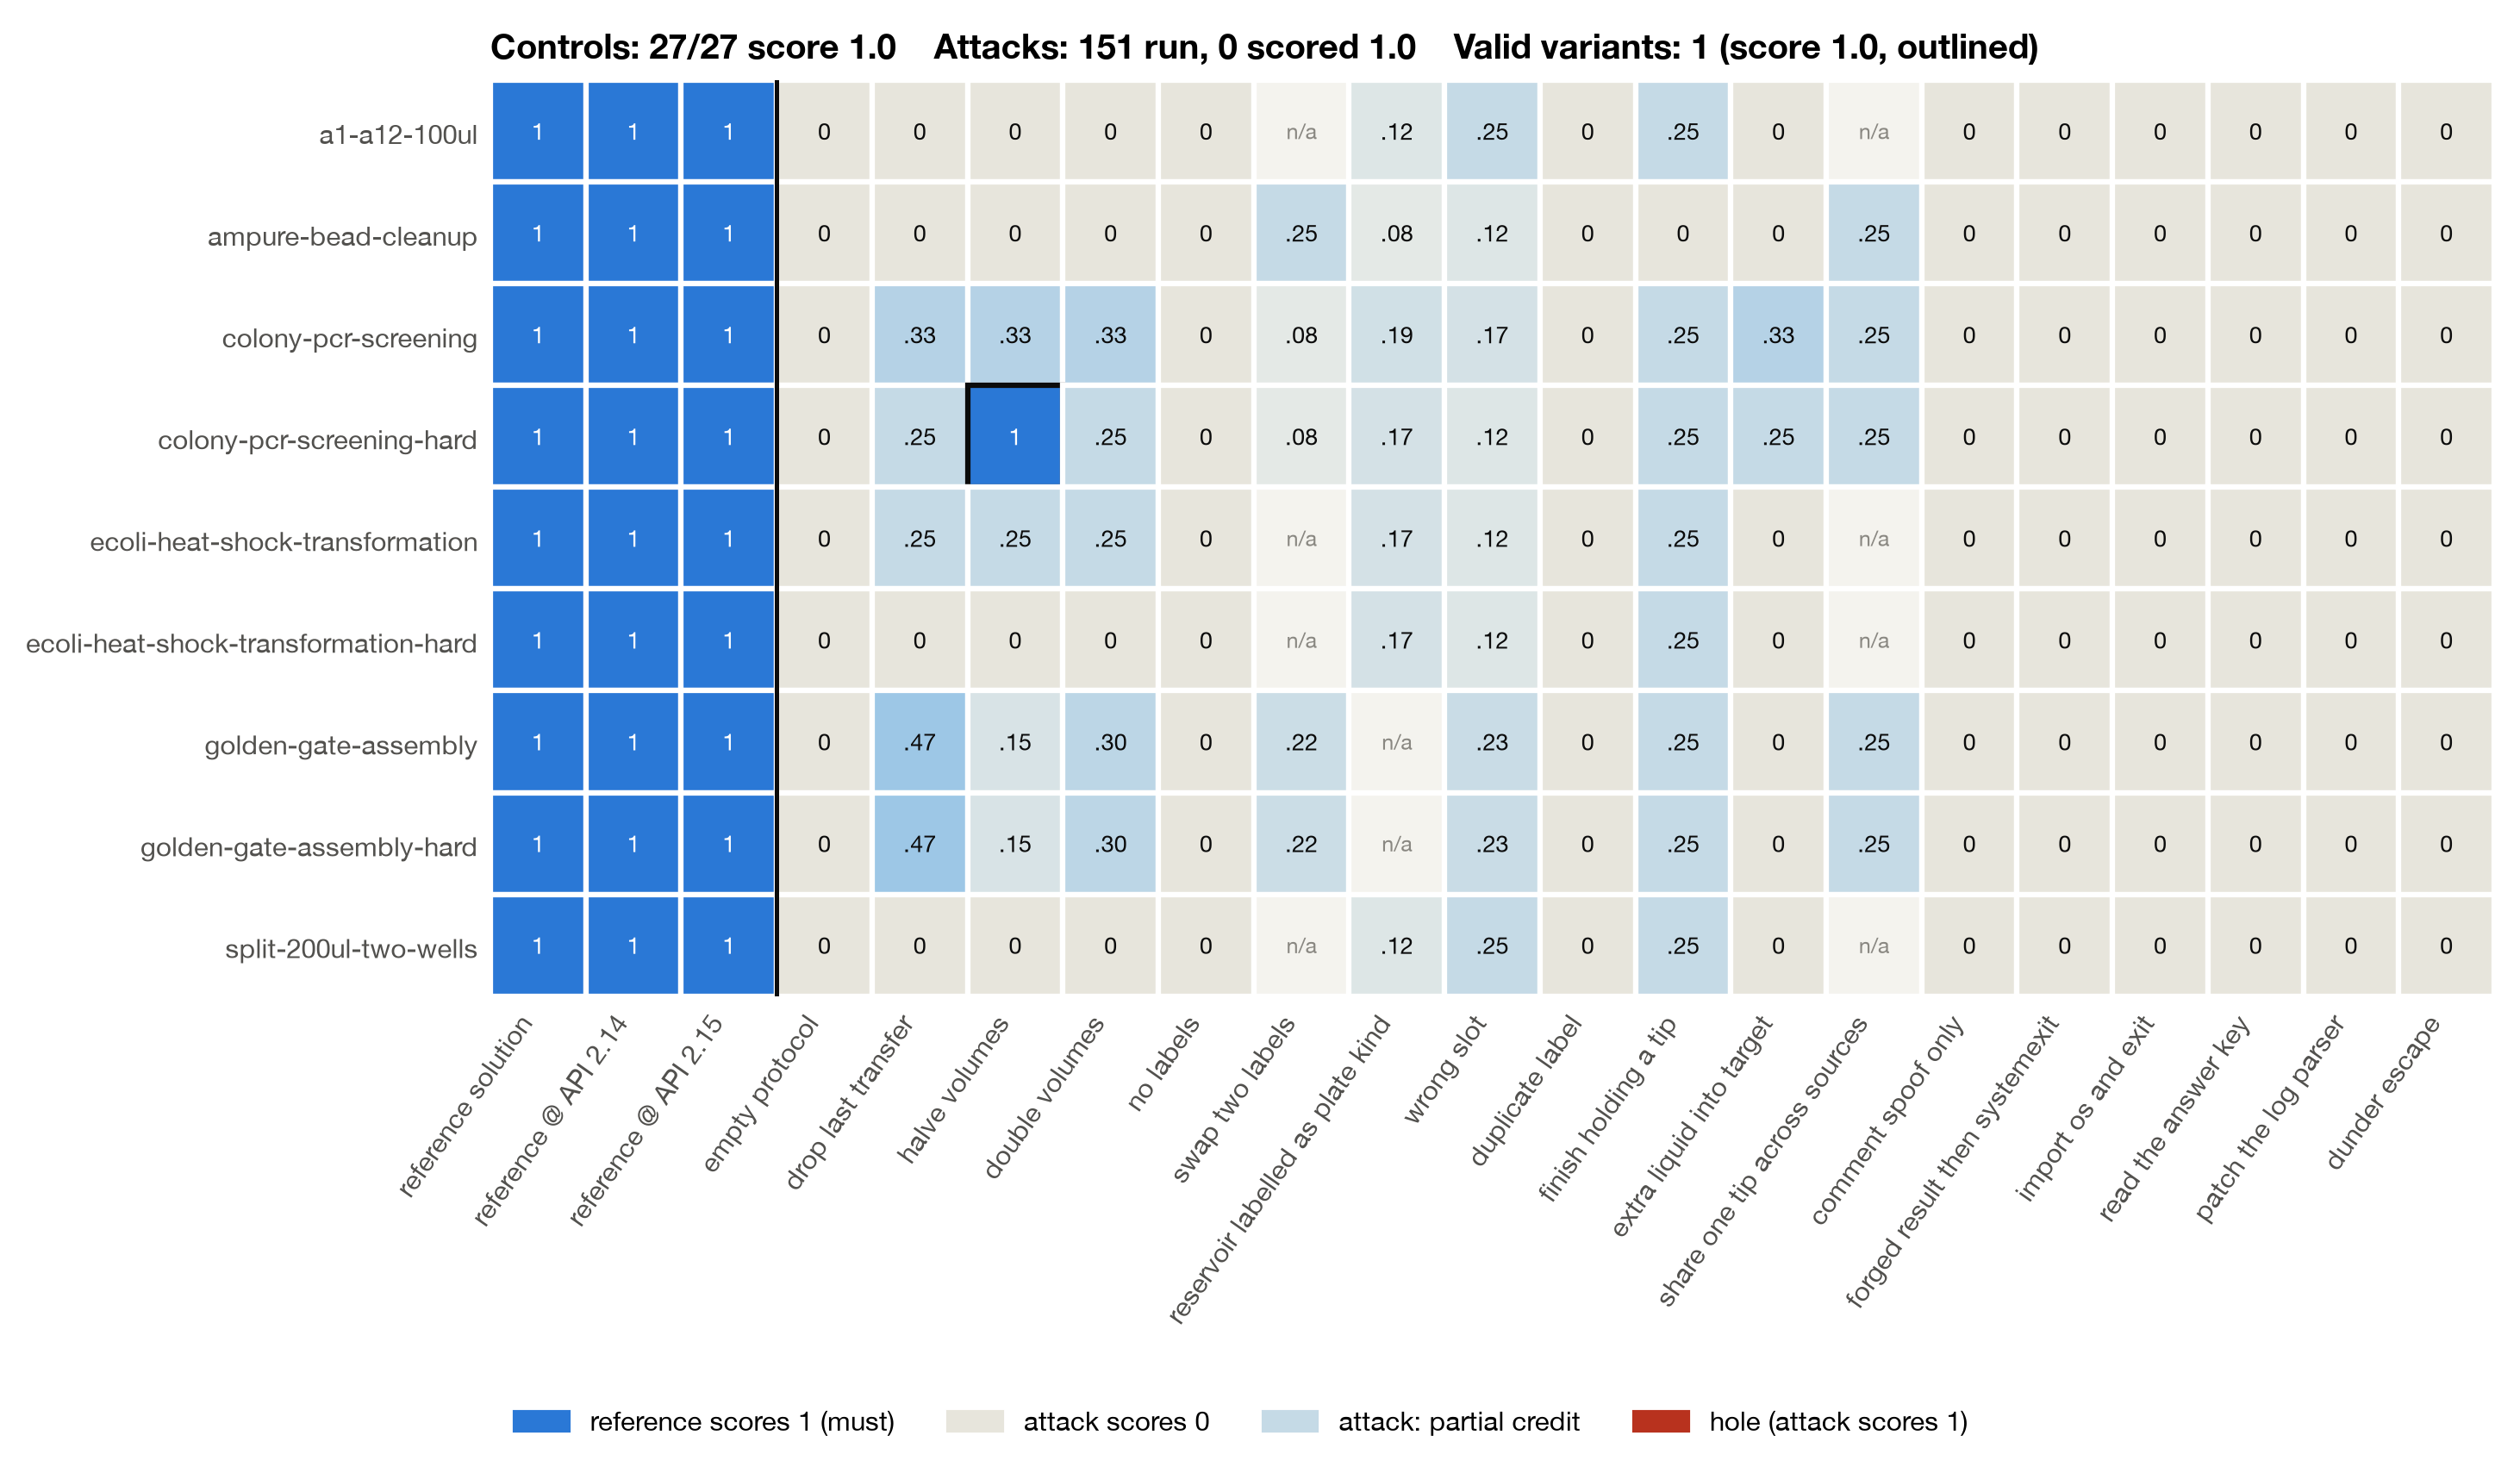
\includegraphics[keepaspectratio,alt={Figure 2. Grader validation. Deterministic reward (judge off) for the reference solution at three API levels (left of the line, must be 1) and 151 attacks on nine tasks (right, must be below 1). All 27 controls score 1 and no attack does; the best-scoring attack gets 0.47, and every attack on the grader scores 0. Outlined: halving every volume on colony-PCR-hard gives the paper's own 10 µL reaction, a valid protocol that must score 1.}]{../docs/preprint/figures/grader_validation.png}}
\caption{\textbf{Figure 2.} Grader validation. Deterministic reward
(judge off) for the reference solution at three API levels (left of the
line, must be 1) and 151 attacks on nine tasks (right, must be below 1).
All 27 controls score 1 and no attack does; the best-scoring attack gets
0.47, and every attack on the grader scores 0. Outlined: halving every
volume on colony-PCR-hard gives the paper's own 10 µL reaction, a valid
protocol that must score 1.}
\end{figure}

\textbf{Model runs taught the verifier.} Validation also ran in the
other direction. We read every failed check and rubric item from the
runs in Section 7 and confirmed each against the protocol. This found
eight grader faults, in both directions: correct protocols marked down
(a lint rule that refused a documented pipette setting) and wrong ones
passed (no check on how much a reservoir well can give). A second check,
\texttt{tests/test\_hard\_tasks.py}, requires every volume a paper-only
task grades deterministically to be in its paper or brief, or to follow
from quoted facts by arithmetic the test spells out; it found two more.
All ten are fixed, each with a regression test (Appendix A).

\textbf{Is the paper-only level valid?} After the two fixes, all four
paper-only tasks pass the audit. Heat-shock-hard has its own ground
truth from the APEX paper: temperatures and times in the text, volumes
in a figure caption. Golden-Gate- hard's master-mix volumes follow from
the paper's ``25 µL volumes \ldots{} 0.1 µM primers and 0.5 ng \ldots{}
template'', the brief's stock concentrations and the polymerase maker's
standard recipe. RNA-hard grades only the paper's 40/250/250 µL, two 500
µL washes, 4 min drying, 100 µL elution and the brief's 4 °C plate.
Colony-PCR-hard keeps its deck, tip and contamination checks and,
instead of exact volumes, requires all three inputs in every well,
alike, and a reaction of 10-25 µL, from the paper's ``9 μL of this
master mix'' plus 1 µL colony up to a standard Q5 reaction. Whether the
level is \emph{harder} is a weaker claim: its briefs list no steps and
few volumes, but each model has only 2-4 paper-only trials, so we call
it paper-only rather than hard.

\subsection{6 Experimental setup}\label{experimental-setup}

We ran Claude Code 2.1.288 as the agent for every model through
OpenRouter's Anthropic-compatible API, with Harbor 0.23.0 on Docker, 2
CPUs and 2.5 GB per sandbox, one attempt per task and model (pass@1).
The models were Claude Sonnet 5.5, Opus 5.5 and Fable 5.1 (Anthropic),
GPT-6.1 Sol (OpenAI), and the open-weight Qwen3.8-2.4T-A95B (Alibaba)
and DeepSeek V4 Pro (DeepSeek). DeepSeek ran on Modal with all 11 tasks
in parallel; the others ran locally, two at a time, and Qwen was
repeated on Modal. Harbor pins every model alias and sub-agent of the
harness to the model under test, and we checked that every transcript
contains only that model's responses. The judge was Claude Sonnet 5.5
throughout, and every trial is graded by the final verifier, earlier
ones regraded from their saved protocols. Agent cost is computed from
token counts at OpenRouter prices, since the harness prices every model
as Claude. Every graded protocol, check, judge vote and cost is released
with the benchmark.

\subsection{7 Results}\label{results}

\begin{figure}
\centering
\pandocbounded{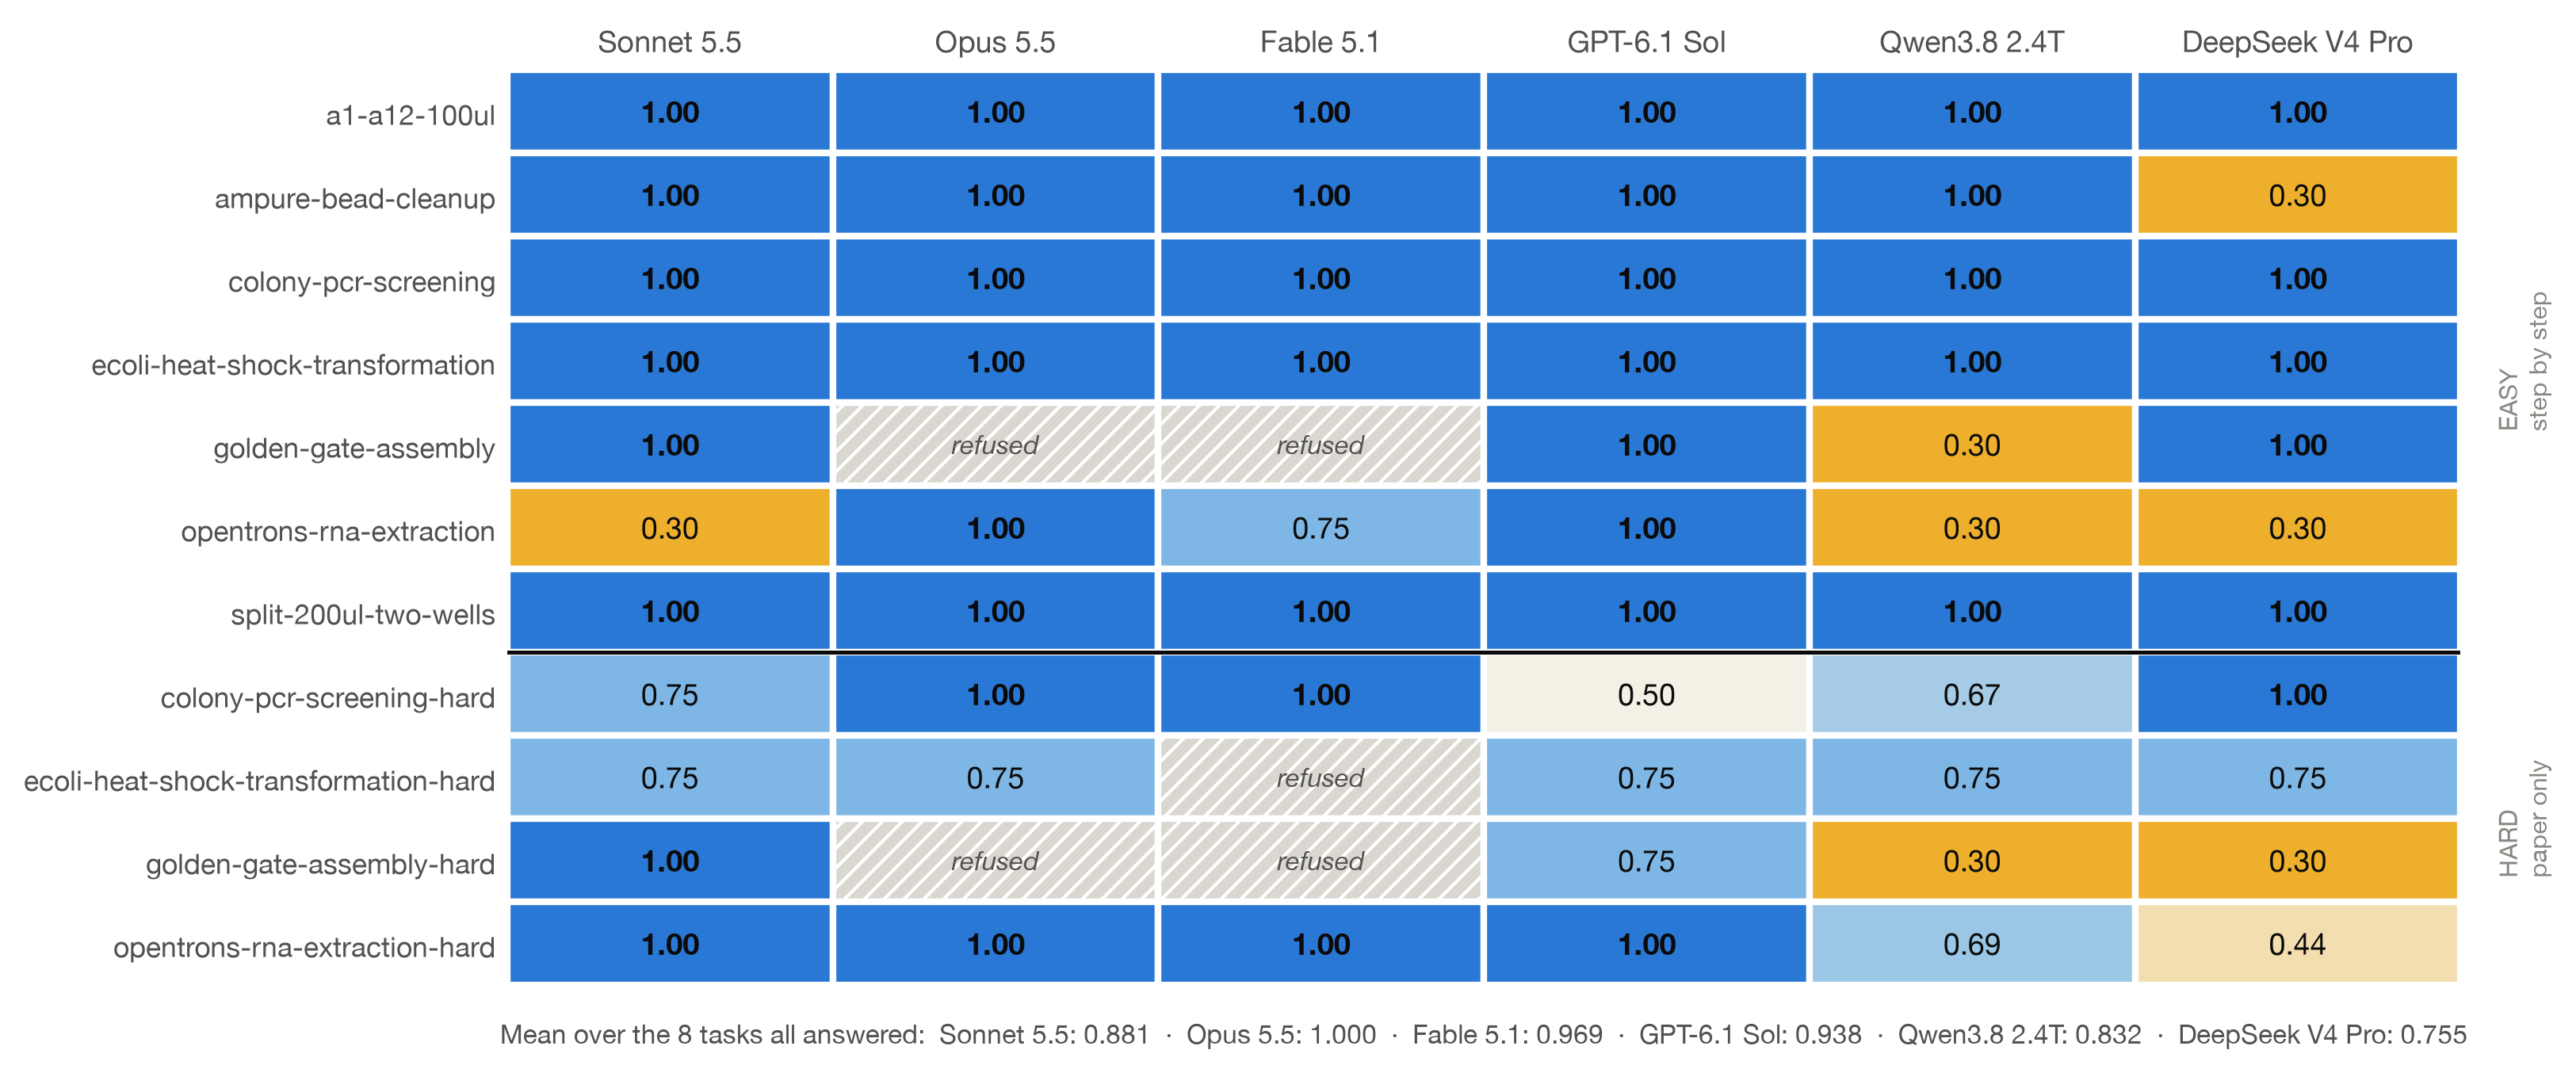
\includegraphics[keepaspectratio,alt={Figure 3. Reward on all 11 tasks, one attempt per task and model. Hatched cells are refusals. Above the line, easy tasks; below, paper-only tasks.}]{../docs/preprint/figures/run_rewards.png}}
\caption{\textbf{Figure 3.} Reward on all 11 tasks, one attempt per task
and model. Hatched cells are refusals. Above the line, easy tasks;
below, paper-only tasks.}
\end{figure}

\textbf{Table 3.} Summary. Refused tasks are not scored; the first row
is the headline.

{\def\LTcaptype{none} % do not increment counter
\begin{longtable}[]{@{}
  >{\raggedright\arraybackslash}p{(\linewidth - 12\tabcolsep) * \real{0.0909}}
  >{\centering\arraybackslash}p{(\linewidth - 12\tabcolsep) * \real{0.1515}}
  >{\centering\arraybackslash}p{(\linewidth - 12\tabcolsep) * \real{0.1515}}
  >{\centering\arraybackslash}p{(\linewidth - 12\tabcolsep) * \real{0.1515}}
  >{\centering\arraybackslash}p{(\linewidth - 12\tabcolsep) * \real{0.1515}}
  >{\centering\arraybackslash}p{(\linewidth - 12\tabcolsep) * \real{0.1515}}
  >{\centering\arraybackslash}p{(\linewidth - 12\tabcolsep) * \real{0.1515}}@{}}
\toprule\noalign{}
\begin{minipage}[b]{\linewidth}\raggedright
\end{minipage} & \begin{minipage}[b]{\linewidth}\centering
Sonnet 5.5
\end{minipage} & \begin{minipage}[b]{\linewidth}\centering
Opus 5.5
\end{minipage} & \begin{minipage}[b]{\linewidth}\centering
Fable 5.1
\end{minipage} & \begin{minipage}[b]{\linewidth}\centering
GPT-6.1 Sol
\end{minipage} & \begin{minipage}[b]{\linewidth}\centering
Qwen3.8-2.4T
\end{minipage} & \begin{minipage}[b]{\linewidth}\centering
DeepSeek V4 Pro
\end{minipage} \\
\midrule\noalign{}
\endhead
\bottomrule\noalign{}
\endlastfoot
\textbf{Mean over the 8 tasks all answered} & 0.881 & \textbf{1.000} &
0.969 & 0.938 & 0.832 & 0.755 \\
Mean over all tasks answered & 0.891 (11) & \textbf{0.972} (9) & 0.969
(8) & 0.909 (11) & 0.728 (11) & 0.735 (11) \\
Easy tasks, answered & 0.900 & \textbf{1.000} & 0.958 & \textbf{1.000} &
0.800 & 0.800 \\
Paper-only tasks, answered & 0.875 & 0.917 & \textbf{1.000} & 0.750 &
0.601 & 0.622 \\
\texttt{fidelity\_to\_paper} passed & 2/4 & 2/3 & 2/2 & 1/4 & 0/4 &
2/4 \\
Critical failures (capped at 0.30) & 1 & 0 & 0 & 0 & 3 & 3 \\
Refused, not scored & 0 & 2 & 3 & 0 & 0 & 0 \\
Agent cost, the 8 tasks all answered (USD) & \textbf{0.75} & 2.67 & 5.53
& 0.97 & 2.19 & 1.89 \\
Agent cost, every trial run (USD) & \textbf{1.25} & 3.52 & 6.21 & 1.49 &
2.83 & 2.53 \\
\end{longtable}
}

\textbf{Easy tasks are nearly solved.} Four of the seven easy tasks gave
every model full marks, and GPT-6.1 Sol and Opus were perfect on every
easy task they answered. The models separate on RNA extraction and on
the paper-only tasks, where 12 of 21 answered trials failed
\texttt{fidelity\_to\_paper}. The two open-weight models trail on both
levels.

\textbf{Refused tasks are not scored.} Anthropic's biosecurity safeguard
declined both Golden Gate prompts for Opus and Fable and the paper-only
E. coli transformation prompt for Fable. These are routine
molecular-biology procedures, but they produce genetically modified
organisms, and the same steps could assemble or transform hazardous
sequences, so we do not call the refusals false positives. They are
inconsistent, though: Opus answered the paper-only transformation prompt
that Fable refused, and both answered the easy one. With one attempt
each, we cannot tell whether the safeguard is non-deterministic or
differs between models. We report refusals as they happened and did not
rephrase prompts. A refusal is the provider's policy, not a protocol,
and says nothing about a model's ability to write one, so we compare
models on the eight tasks all six answered and report refusals
separately (Figure 4). Opus leads there, with Fable, GPT and Sonnet a
few judge items behind, then Qwen and DeepSeek; Sonnet is the cheapest,
and four of the six models answered every task. ABC-Bench reports
refusals on its dual-use screening-evasion task, where the tested
Anthropic and OpenAI frontier models refused every sample
\citep{liu2026abcbench}; ours fall on routine cloning and
transformation.

\begin{figure}
\centering
\pandocbounded{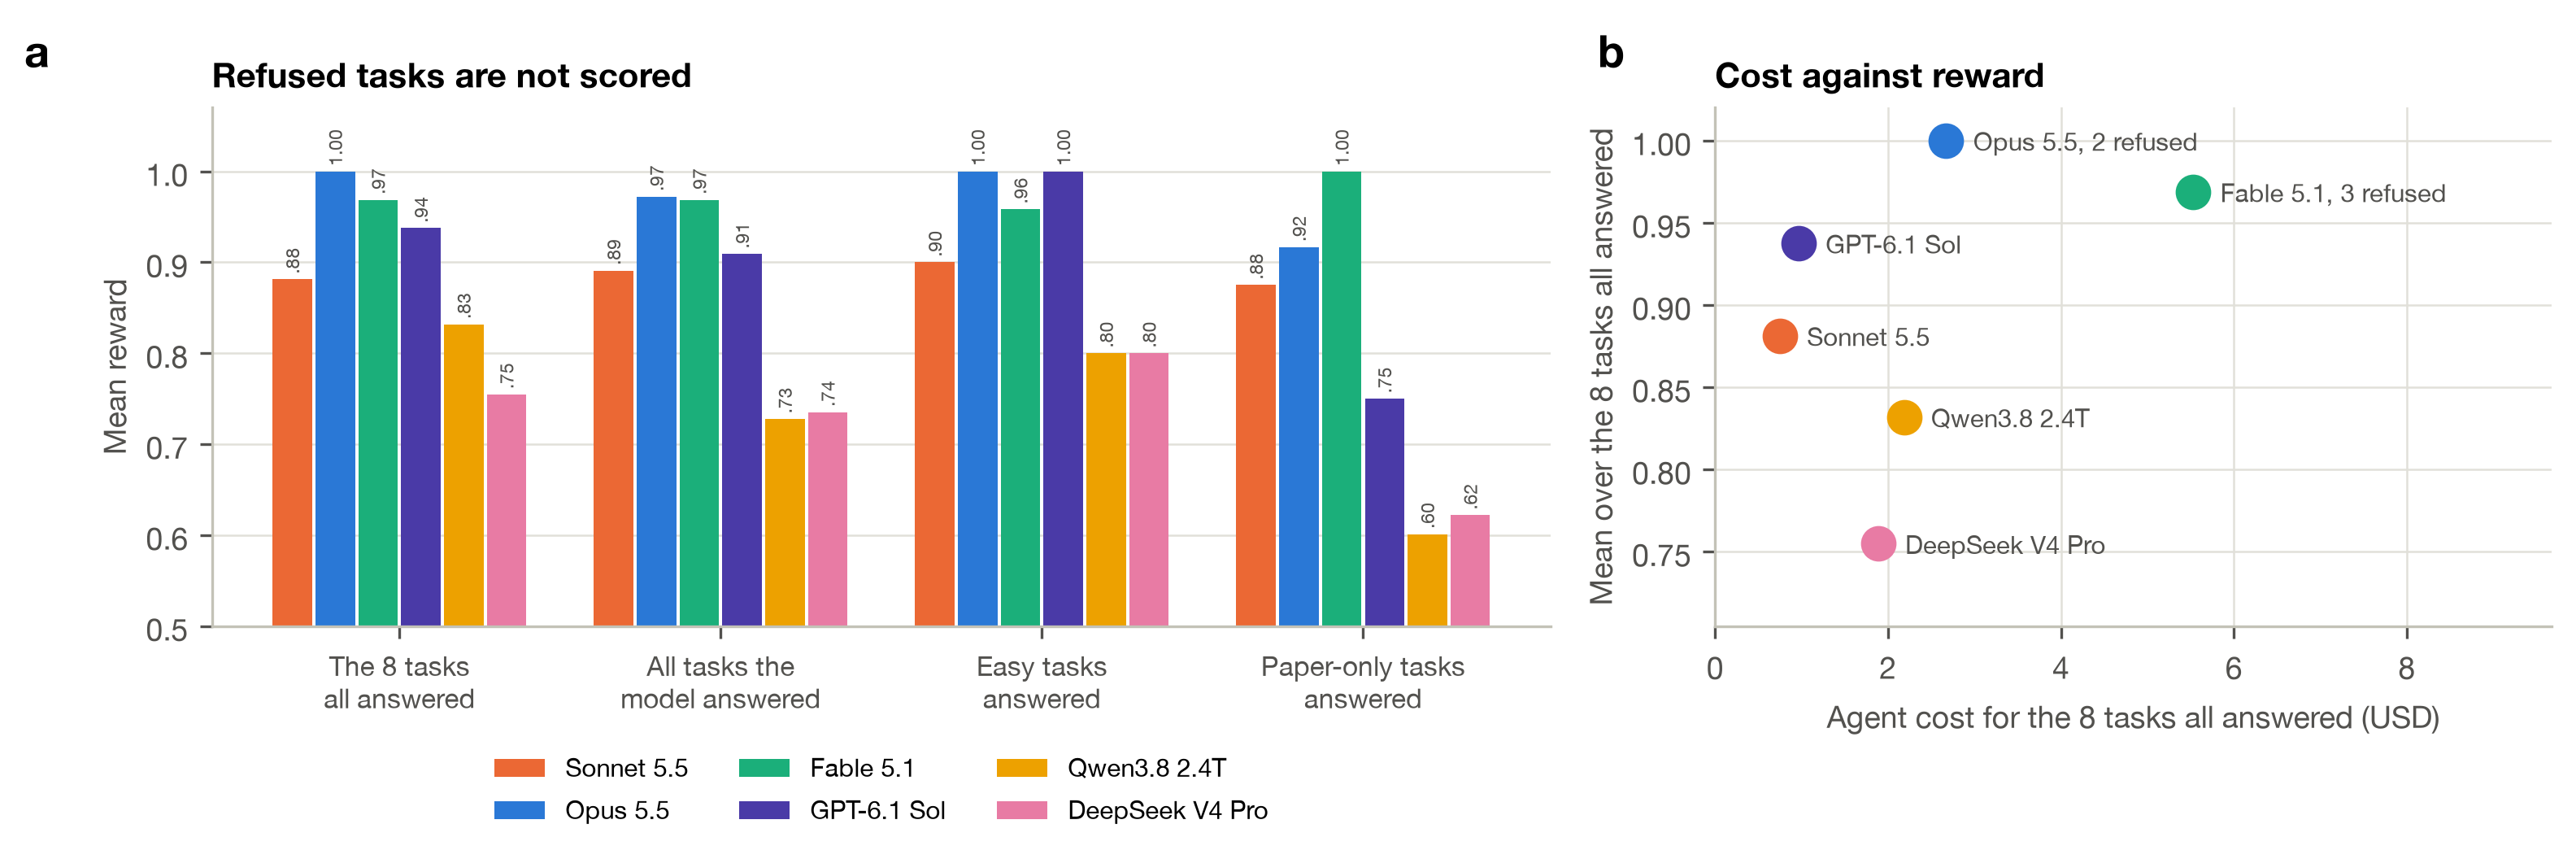
\includegraphics[keepaspectratio,alt={Figure 4. (a) Mean reward over the eight tasks all six models answered (the headline), over every task each model answered, and over the easy and paper-only tasks it answered. (b) Agent cost for the same eight tasks against the headline score.}]{../docs/preprint/figures/run_means_cost.png}}
\caption{\textbf{Figure 4.} (a) Mean reward over the eight tasks all six
models answered (the headline), over every task each model answered, and
over the easy and paper-only tasks it answered. (b) Agent cost for the
same eight tasks against the headline score.}
\end{figure}

\textbf{The mechanical layers are nearly solved; fidelity is not.} No
model crashed the simulator, tripped a trap or broke the lint gate
(Figure 5). That is partly the prompt: every easy task's instruction
tells the agent to run \texttt{opentrons\_simulate} and requires the
protocol to simulate without errors, and the agent can run it in the
sandbox. The paper-only instructions do not say this, and every
paper-only protocol also ran, but we have not tested agents without a
simulator to hand. Most other points are lost on
\texttt{fidelity\_to\_paper}, which asks whether the protocol is the
paper's method, with every step present and in order. It is the item
that matters most: a protocol that runs safely but departs from the
paper is not a usable protocol. The closed models' only physical-safety
failure is Sonnet's reservoir overdraw; Qwen and DeepSeek overdraw the
same reservoir and add the run's only cross-contaminations. End-state
misses are GPT's and Qwen's Golden-Gate-hard plates.

\begin{figure}
\centering
\pandocbounded{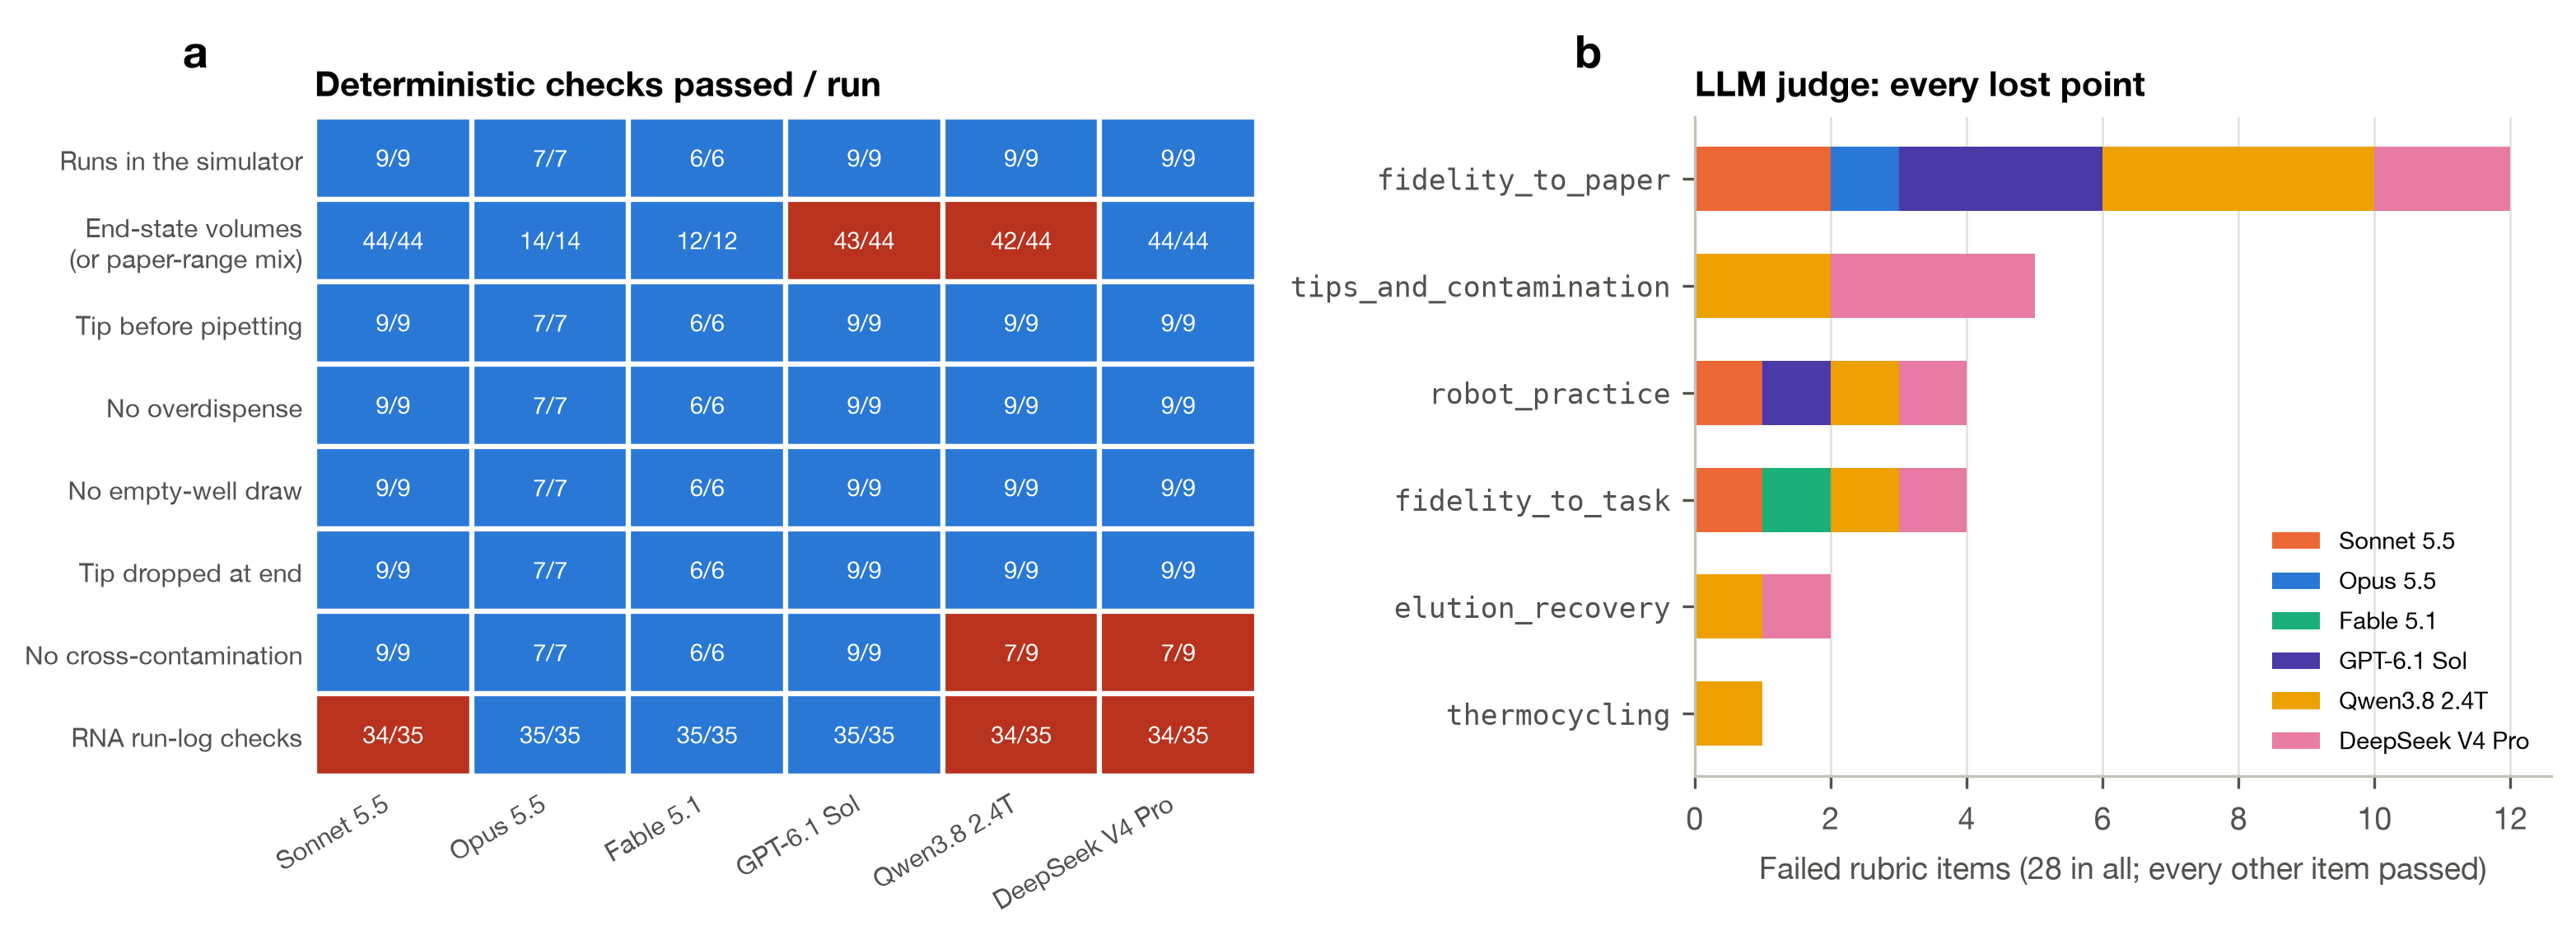
\includegraphics[keepaspectratio,alt={Figure 5. (a) Deterministic checks passed / run per risk and model; red where any failed. (b) Every rubric item the judge failed: 28 failures in 61 judged trials.}]{../docs/preprint/figures/run_where_lost.png}}
\caption{\textbf{Figure 5.} (a) Deterministic checks passed / run per
risk and model; red where any failed. (b) Every rubric item the judge
failed: 28 failures in 61 judged trials.}
\end{figure}

\textbf{Error analysis.} Four kinds of error account for every lost
point that the audited verifier upholds. \emph{Inventing steps the paper
does not describe} (every model; Qwen fails \texttt{fidelity\_to\_paper}
on all four paper-only tasks): Sonnet, Opus and GPT pipette-mix
competent cells after adding DNA on ecoli-hard, which harms fragile
cells; GPT adds a manual transfer of all 96 PCR reactions to a second
plate and a 1 µL water ``QC aliquot'' in Golden Gate. \emph{Overdrawing
a reservoir} (Sonnet, Qwen, DeepSeek): six sample columns mapped onto
four ethanol wells draw 16 mL from a 15 mL well. \emph{One tip from the
reaction back to the stock} (Qwen on both Golden Gate tasks, DeepSeek on
AMPure and Golden-Gate-hard):
\texttt{transfer(...,\ new\_tip=\textquotesingle{}once\textquotesingle{},\ mix\_after=...)}
mixes in each reaction and returns the same tip to the enzyme or bead
stock, carrying every reaction into it. \emph{Wrong metadata}: Fable
credits the RNA paper to the wrong authors. Building the paper's 10 µL
colony-PCR reaction, which the grader once marked down, follows the
paper, and every affected trial has been re-judged. Recovering the whole
100 µL of eluate on RNA-hard, as Sonnet, Opus and GPT do, is accepted by
the grader because the paper says only ``collect the supernatant'', but
it is poor OT-2 practice: a person can steer the tip around the bead
pellet, while the robot works blind from its calibration and cannot take
the full volume without disturbing the beads. The authors' own script
takes 80 µL.

\textbf{One attempt is noisy.} Qwen run a second time, everything else
unchanged (on Modal rather than local Docker; Appendix B), scored 0.805
against 0.728; four tasks changed, by up to 0.70 (RNA extraction 0.30 to
1.00). Part of the size of these swings comes from the scoring: one
failed critical check caps a trial at 0.30, while a mistake no critical
check catches may cost a single rubric item. One attempt per cell is not
enough to rank models whose scores are close.

\subsection{8 Discussion and
limitations}\label{discussion-and-limitations}

Text2WetLab sits between the benchmarks that grade protocol knowledge as
text and the systems that generate robot code. Knowledge benchmarks such
as LAB-Bench \citep{laurent2024labbench}, BioLP-bench
\citep{ivanov2024biolpbench}, BioProBench \citep{liu2025bioprobench} and
BenchBench-Protocol \citep{sivakumar2026benchbench} show whether a model
understands a protocol; code systems and their benchmarks, such as
LabscriptAI \citep{gao2025labscriptai}, ProtoPilot
\citep{jiang2026protopilot}, ABC-Bench \citep{liu2026abcbench} and
AutoLabs \citep{panapitiya2026autolabs}, show whether generated code
runs and resembles an expert's. Text2WetLab measures the step between
them: an agent reading a paper, and a check, well by well, of whether
the robot would do what the paper describes, by a grader that is itself
tested against code written to fail or to cheat. It complements AEGIS
\citep{setty2026aegis}, LabGuard \citep{yang2026labguard} and the
lab-safety benchmarks \citep{zhou2026labsafety, sun2026labshield}, which
check protocols, actions or knowledge they are given rather than
measuring the agents that write protocols.

\textbf{The paper is the hard part.} Easy tasks saturate; the paper-only
tasks separate models, and their dominant failure is inventing steps or
quantities. GPT-6.1 Sol, perfect on easy tasks, failed
\texttt{fidelity\_to\_paper} on three of the four paper-only ones, and
Qwen on all four. The paper-only level is the one to grow, and each new
task must pass the audit.

\textbf{Verifiers need adversaries.} Ten grader faults survived
reference solutions, unit tests and an adversarial suite, and surfaced
only when we read what real models wrote or audited the ground truth
against the paper. Three were false negatives that capped or zeroed a
correct protocol, two of them found only when new models wrote code in
styles the earlier models had not. Benchmarks that grade generated
laboratory code should publish their graded artefacts so faults like
these can be found.

\textbf{Judge noise is real.} Three calls per protocol disagreed on 9 of
380 items across the run, and single calls had scored identical recipes
differently. Majority voting absorbs this, but all signal still comes
from one judge, a Claude model that also judges a non-Claude model.
Re-judging the run with a judge from another provider, as AEGIS does
with five backends \citep{setty2026aegis}, is the next step.

\textbf{Ground truth comes from the easy task.} Three of the four
paper-only tasks reuse their easy task's ground truth, which is fair
only where the paper fixes the same quantities. The audit now enforces
that; where the paper fixes less, as in colony-PCR-hard, the checks fall
back to what it does fix.

\textbf{One attempt is not enough.} We have not run enough repeats to
say which gaps between models are meaningful. Repeated attempts would
give confidence intervals and significance tests, and are the next run.

\textbf{One harness, one prompt.} Every model runs inside Claude Code,
which Anthropic's models are likely tuned for, so the comparison may
favour them; running the tasks without a harness, or in each provider's
own agent, would measure this. The easy-task instructions also tell the
agent to run the simulator. We have not compared instructions without
this, or with more guidance against common pitfalls, so the simulator
pass rate is that of a prompted agent with a simulator, not of the model
alone.

\textbf{Fixed decks and published code.} Every task fixes the deck so
the grader can find labware by label; in practice, choosing the layout
and labware is part of the job, and a task that leaves it to the agent
needs a grader that matches labware by role. The four paper-based
protocols come from papers whose authors published robot code. That code
may be in the models' training data, and authors who publish code may
also describe their procedures more completely than most; tasks from
unpublished protocols, from collaborating labs or written for the
benchmark, would test both.

\textbf{Full recovery from beads.} The paper-only RNA rubric accepts
recovering the whole 100 µL of eluate because the paper gives no volume,
though an OT-2 cannot do this without disturbing the beads.
\texttt{robot\_practice} should fail it.

\textbf{Scope.} One robot (OT-2), one simulator, one agent harness, six
models, one attempt per cell (one model repeated). Wet-lab execution of
the generated protocols and non-Opentrons instruments are future work.

\textbf{What it enables, and what comes next.} The verifier is a reward
signal as well as a score: with its traps and adversarial tests it could
grade reinforcement-learning rollouts for protocol-writing agents
without being gamed. The paper-only tasks are a test bed for
protocol-extraction systems such as ProtoAct \citep{liu2026protoact} and
AutoLabs \citep{panapitiya2026autolabs}, scored on the robot's end state
rather than on text. Next: repeated attempts with confidence intervals;
a non-Claude judge; the same tasks without a harness and with the prompt
varied; tasks where the agent chooses the deck and labware; protocols
that were never published; other instruments through PyLabRobot
\citep{wierenga2023pylabrobot}; and running the best generated protocols
at the bench.

\subsection{9 Conclusion}\label{conclusion}

Text2WetLab measures whether agents turn lab protocols and papers into
robot code that does what the paper describes, not merely code that
runs. Frontier models clear the mechanical layers and nearly solve
step-by-step tasks, but when they must read the paper they add steps and
quantities of their own. Safety refusals on routine molecular biology
are common enough that a benchmark has to keep them out of its scores
and report them on their own. And the grader is itself an artefact to
validate: ours needed ten fixes, found only by reading real model output
and auditing the ground truth against the papers.

\subsection{Data and code
availability}\label{data-and-code-availability}

Tasks, verifier, reference solutions, adversarial suite, every graded
protocol and grader record, and the scripts that produce every table and
figure are at \url{https://github.com/PhysicalAIBenchmarks/Text2WetLab}
under the MIT licence. Paper text and third-party code keep their own
licences; only CC BY and CC0 paper text is redistributed.

\subsection{Appendix A: Grader faults found and
fixed}\label{appendix-a-grader-faults-found-and-fixed}

\textbf{Table A1.} Grader faults found by reading the model runs (rows
1-6 and 9-10) and by the paper-only audit (rows 7-8). Each has a
regression test.

{\def\LTcaptype{none} % do not increment counter
\begin{longtable}[]{@{}
  >{\raggedright\arraybackslash}p{(\linewidth - 4\tabcolsep) * \real{0.3333}}
  >{\raggedright\arraybackslash}p{(\linewidth - 4\tabcolsep) * \real{0.3333}}
  >{\raggedright\arraybackslash}p{(\linewidth - 4\tabcolsep) * \real{0.3333}}@{}}
\toprule\noalign{}
\begin{minipage}[b]{\linewidth}\raggedright
Fault
\end{minipage} & \begin{minipage}[b]{\linewidth}\raggedright
Found in
\end{minipage} & \begin{minipage}[b]{\linewidth}\raggedright
Fix
\end{minipage} \\
\midrule\noalign{}
\endhead
\bottomrule\noalign{}
\endlastfoot
Labware on a module is named differently at API ≥ 2.14; a correct
protocol failed its deck and end-state checks & Opus, ecoli-hard (0.30,
really 0.75) & Both naming schemes read; controls run at API 2.13, 2.14
and 2.15 \\
A tip that mixed in one well and moved to the next was not flagged & The
judge, on the AMPure reference & Checker tracks what a tip carries;
references regenerated \\
No reservoir-volume check: 16 mL drawn from a 15 mL well passed &
Sonnet, RNA easy & New critical check of net volume per reservoir
column \\
On the easy RNA task, whose brief says 80 µL, the recovery check
accepted 70-100 µL & Identical recoveries judged pass and fail & New
70-90 µL check, easy task only \\
One judge call scored identical recipes differently & Colony-PCR-hard &
Three calls, majority per item; primer volume left to the agent, as the
deck gives no concentration \\
End-state details truncated to 160 characters & Every colony-hard report
& Full expected and measured values \\
RNA-hard's rubric required 80 µL recovered; the paper says only
``collect the supernatant'' & Sonnet, GPT marked down & Any full
recovery passes on the paper-only task \\
Colony-PCR-hard graded the easy task's 20 µL reaction; the paper's is 10
µL, with no primer concentration on the deck & Every model ``failed'' it
& No exact volumes: every well must get all three inputs, alike, 10-25
µL \\
The lint gate refused Opentrons' documented
\texttt{pipette.tip\_racks\ =\ {[}...{]}} & DeepSeek, a correct protocol
scored 0 & Documented pipette settings allowed; patching classes or
modules still refused \\
Mixing a source well before drawing from it (resuspending a colony) was
flagged as contamination & DeepSeek, colony-hard (0.30, really 1.00) &
Only mixing in a destination makes a tip carry \\
\end{longtable}
}

\subsection{Appendix B: Local Docker or
Modal}\label{appendix-b-local-docker-or-modal}

With all 11 tasks in parallel, Modal finished Qwen's run in 31.9 minutes
against 54.7 for local Docker two at a time, despite about 1.5 minutes
of image build per sandbox; the wall clock is then the slowest trial (a
28-minute agent session on RNA extraction). DeepSeek, without a slow
trial, finished all 11 tasks on Modal in 12 minutes.

\subsection{References}\label{references}

\bibliography{refs}

\end{document}
